\chapter{Contesto aziendale}
\label{chap:contesto-aziendale}

% Descrizione generale dell'azienda che mi ha ospitato nel mio periodo di \textit{stage}.
\section{L'azienda}\label{sec:the-company}\noindent
M31 S.r.l. è un'azienda italiana nata nel 2007 con sede a Padova.
Essa si specializza in ingegneria all'avanguardia su una variegata gamma di ambiti, come ad esempio: \textit{mechanical \& robotics}, \textit{software engineering}, \textit{artificial intelligence}, \textit{IoT} e molto altro.
L'azienda affianca i suoi clienti con cui svolge progetti, partendo dalla fase esplorativa fino alla fase di industrializzazione e certificazione.
Nei diciasette anni di operazione, M31 ha realizzato più di cento unici progetti di innovazione che hanno avantaggiato proprie startup, imprese del territorio e grandi gruppi.

% Descrizione dei vari clienti con cui l'azienda collabora.
\section{Tipologia di clientela}\label{sec:client-types}\noindent
La clientela di M31 è abbastanza variegata, ma i settori in cui opera e ha operato sono:
\begin{itemize}
    \item \textbf{Biomedicina:} per la creazione di strumenti diagnostici, piattaforme di \textit{liquid handling} e sistemi di monitoraggio remoto.
    \item \textbf{Monitoraggio e Sicurezza:} sistemi che variano da monitoraggio, antintrusione, videosorveglianza e sensori di allarme.
    \item \textbf{Applicazioni industriali:} per l'evoluzione di processi produttivi, in ambiti come quello delle lavorazioni meccaniche o tessili.
    \item \textbf{\textit{Automation} \& \textit{smart cities}:} per l'automatizzazione di processi in vari ambienti, che siano domestico, di assistenza sanitaria oppure di processi fotografici.
    \item \textbf{\textit{Cloud} \& \textit{digital twins}:} lo sviluppo di una controparte digitale di un prodotto o processo sul \textit{cloud}.
    \item \textbf{\textit{Racing} \& \textit{automotive}:} nell'ambito di vari sistemi e della telemetria per vari sport.
\end{itemize}

% Raffigurazione della struttura interna aziendale.
\section{Organizzazione aziendale}\label{sec:company-organization}\noindent
L'organizzazione aziendale di M31 è suddivisa in diversi settori, questi sono: \textit{governance}, \textit{R\&D team}, \textit{marketing \& sales} e \textit{procurement \& supply chain}.
\subsubsection*{Governance}\noindent
Questo settore si occupa di amministrare l'azienda, questo avviene in vari modi: presa di decisioni per la direzione dell'azienda, gestione e manutenzione delle risorse finanziarie e la gestione e organizzazione del capitale umano.\\
I ruoli che possiamo trovare in questo ramo sono principalmente: il \textit{CEO}, anche chiamato amministratore delegato, \textit{accounting specialist} e \textit{HR manager}.
\subsubsection*{Marketing \& sales}\noindent
Questo è il settore che si occupa di aumentare la visibilità e rapporti con possibili clienti, ma anche di ricercare quali sono le richieste attuali del mercato.\\
Questo \textit{team} non è relativamente grande, nonostante ciò è possibile notare la presenza del \textit{CBO}, anche detto direttore commerciale in lingua italiana.
\subsubsection*{Procurement \& supply chain}\noindent
Questa area aziendale si occupa di far sì che le operazioni aziendali possano procedere in modo adeguato, garantendo l'approvvigionamento delle risorse necessarie e la gestione della catena di fornitura.
\subsubsection*{R\&D team}\noindent
Infine, passiamo al settore aziendale dove sono stato inserito, ovvero il reparto di ricerca e sviluppo. Questo settore è quello più grande dell'azienda, ed è qui che i prodotti effettivi vengono sviluppati.\\
Ci sono varie aree di specializzazione in questo comparto, esse sono divise in una sorta di gruppi di lavoro, che possono o meno coordinarsi per lavorare insieme ai progetti aziendali attualmente in sviluppo.\\
Personalmente sono stato inserito sotto al \textit{team} di \textit{computer vision} e, come ogni altro stagista, anche sotto allo \textit{stage coordinator}.

% Descrizione dei vari processi interni all'azienda,  con un focus specifico sulle metodologie utilizzate per la gestione dei progetti.
\section{Processi aziendali}\label{sec:company-processes}\noindent
Durante il mio periodo di \textit{stage} ho potuto assistere a come vengono gestiti i progetti all'interno dell'azienda. Viene utilizzata la metodologia \textit{Agile}, ma in particolare il \textit{framework} Scrum.
Attraverso questo \textit{framework}, i progetti vengono suddivisi in varie iterazioni denominati \textit{sprint}, ad ognuno di esse, viene assegnata una certa durata di tempo, che può variare da una o più settimane.\\
Ogni \textit{sprint} inizia con un \textit{sprint planning}, nel quale vengono definite le attività da svolgere nello stesso \textit{sprint}, queste attività vengono assegnate ai vari membri dello specifico \textit{team} che si occupa di quel progetto.\\
All'inizio di ogni giornata lavorativa, viene eseguito il \textit{daily stand-up}, nel quale viene discusso il procedimento dei lavori; in particolare viene discusso quello che è stato fatto la giornata precedente e cosa verrà fatto nella giornata attuale.\\
A fine di ogni \textit{sprint} vengono fatti lo \textit{sprint review} e lo \textit{sprint retrospective}, il primo ha la finalità di valutare se tutte le attività sono state svolte e che siano state fatte correttamente, mentre il secondo considera le problematiche riscontrate durante lo \textit{sprint}, definendo possibili miglioramenti al \textit{way of working}, nel caso ne fosse necessario.
\begin{figure}[H]
    \centering
    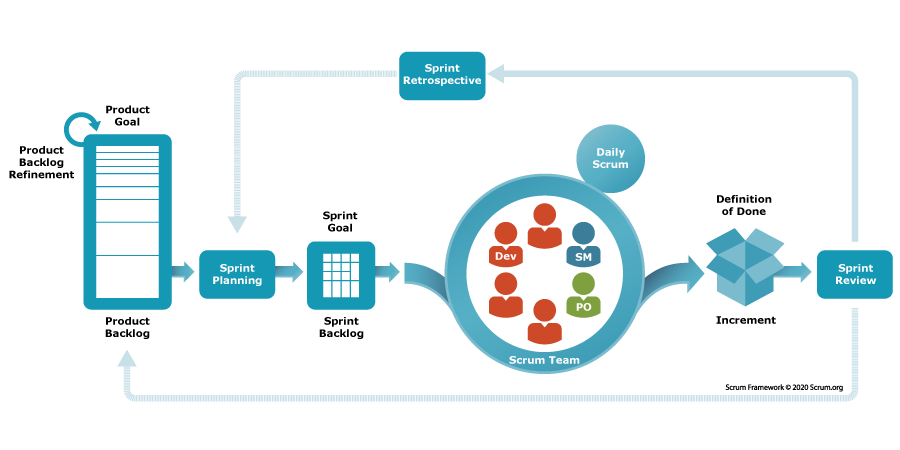
\includegraphics[alt={Rappresentazione del framework Scrum utilizzato in azienda\\ Fonte: scrum.org}, width=0.9\columnwidth]{img/scrum.png}
    \caption[Rappresentazione del \textit{framework} Scrum utilizzato in azienda]{\centering Rappresentazione del \textit{framework} Scrum  utilizzato in azienda \par \textbf{Fonte:} \href{https://www.scrum.org/resources/what-scrum-module}{scrum.org}}
    \label{fig:scrum}
\end{figure}

\section{Tecnologie e strumenti}\label{sec:technologies}

% Lista delle tecnologie utilizzate, descrivendo principalmente le tecnologie utilizzate nella sezione aziendale in cui sono stato inserito, senza menzione di altri progetti a cui non ho partecipato.
\subsection{Tecnologie utilizzate}\noindent
In azienda vengono usate svariate tecnologie, questo è dovuto principalmente dal fatto che vengono svolti più progetti allo stesso tempo. Non avendo familiarità sugli altri progetti, esporrò le tecnologie che furono a me più vicine.
\subsubsection*{Python}\noindent
\textit{Python} è un linguaggio di programmazione ad alto livello, interpretato e di uso generale.
È attualmente il linguaggio più popolare\footnote{Fonte: \href{https://www.tiobe.com/tiobe-index/}{https://www.tiobe.com/tiobe-index/}} al mondo, questo è dovuto dalla semplicità di utilizzo e dal buon supporto di librerie di terze parti, che semplificano ambiti come ad esempio: \textit{web development}, \textit{data science}, \gls{machinelearning} e \textit{scripting} di operazioni ripetitive.
Perciò non stupisce l'utilizzo di questo linguaggio per l'ambito di \textit{machine learning} e per manipolare i \textit{dataset}.
\subsubsection*{TensorFlow}\noindent
\textit{TensorFlow} è una libreria \textit{open-source} sviluppata da \textit{Google} per il \textit{machine learning} e il \gls{deeplearning}.
È una delle librerie più popolari per la creazione e addestramento di modelli basati su tecniche di \textit{machine learning}.
\textit{TensorFlow} integra al suo interno librerie per sfruttare a pieno processori specifici, come ad esempio le \gls{GPU} e le \gls{TPU}, permettendo così di utilizzare risorse computazionali più adeguate, per questo ambito, in modo semplice.
\subsubsection*{Keras}\noindent
Keras è un'altra libreria \textit{open-source} per il \textit{deep learning}, sviluppata per essere semplice e modulare.
Di recente è stata riscritta basandosi su \textit{TensorFlow} e, come quest'ultima, permette di creare e addestrare modelli di intelligenza artificiale, ma rende il processo più rapido e intuitivo.
Keras supporta una variegata tipologia di reti neurali pronte all'uso, come ad esempio reti neurali convoluzionali e ricorrenti, lasciando comunque la possibilità di modificare qualsiasi cosa si voglia adattare meglio alle proprie esigenze.
%Queste caratteristiche rendono questa libreria semplice e potente

% Elenco degli strumenti utilizzati per il supporto i processi, accompagnato da una descrizione del loro scopo e delle loro funzionalità.
\subsection{Strumenti di supporto ai processi}\noindent
\subsubsection*{Jira}\noindent
\textit{Jira} è un software propretario sviluppato da \textit{Atlassian}, è utilizzato come Issue Tracking System (ITS), viene utilizzato per gestire le attività dei vari progetti con la metodologia \textit{Agile}.
All'interno di questo software si possono dedicare delle \textit{board} per i vari \textit{sprint} che vengono svolti.
\begin{figure}[H]
    \centering
    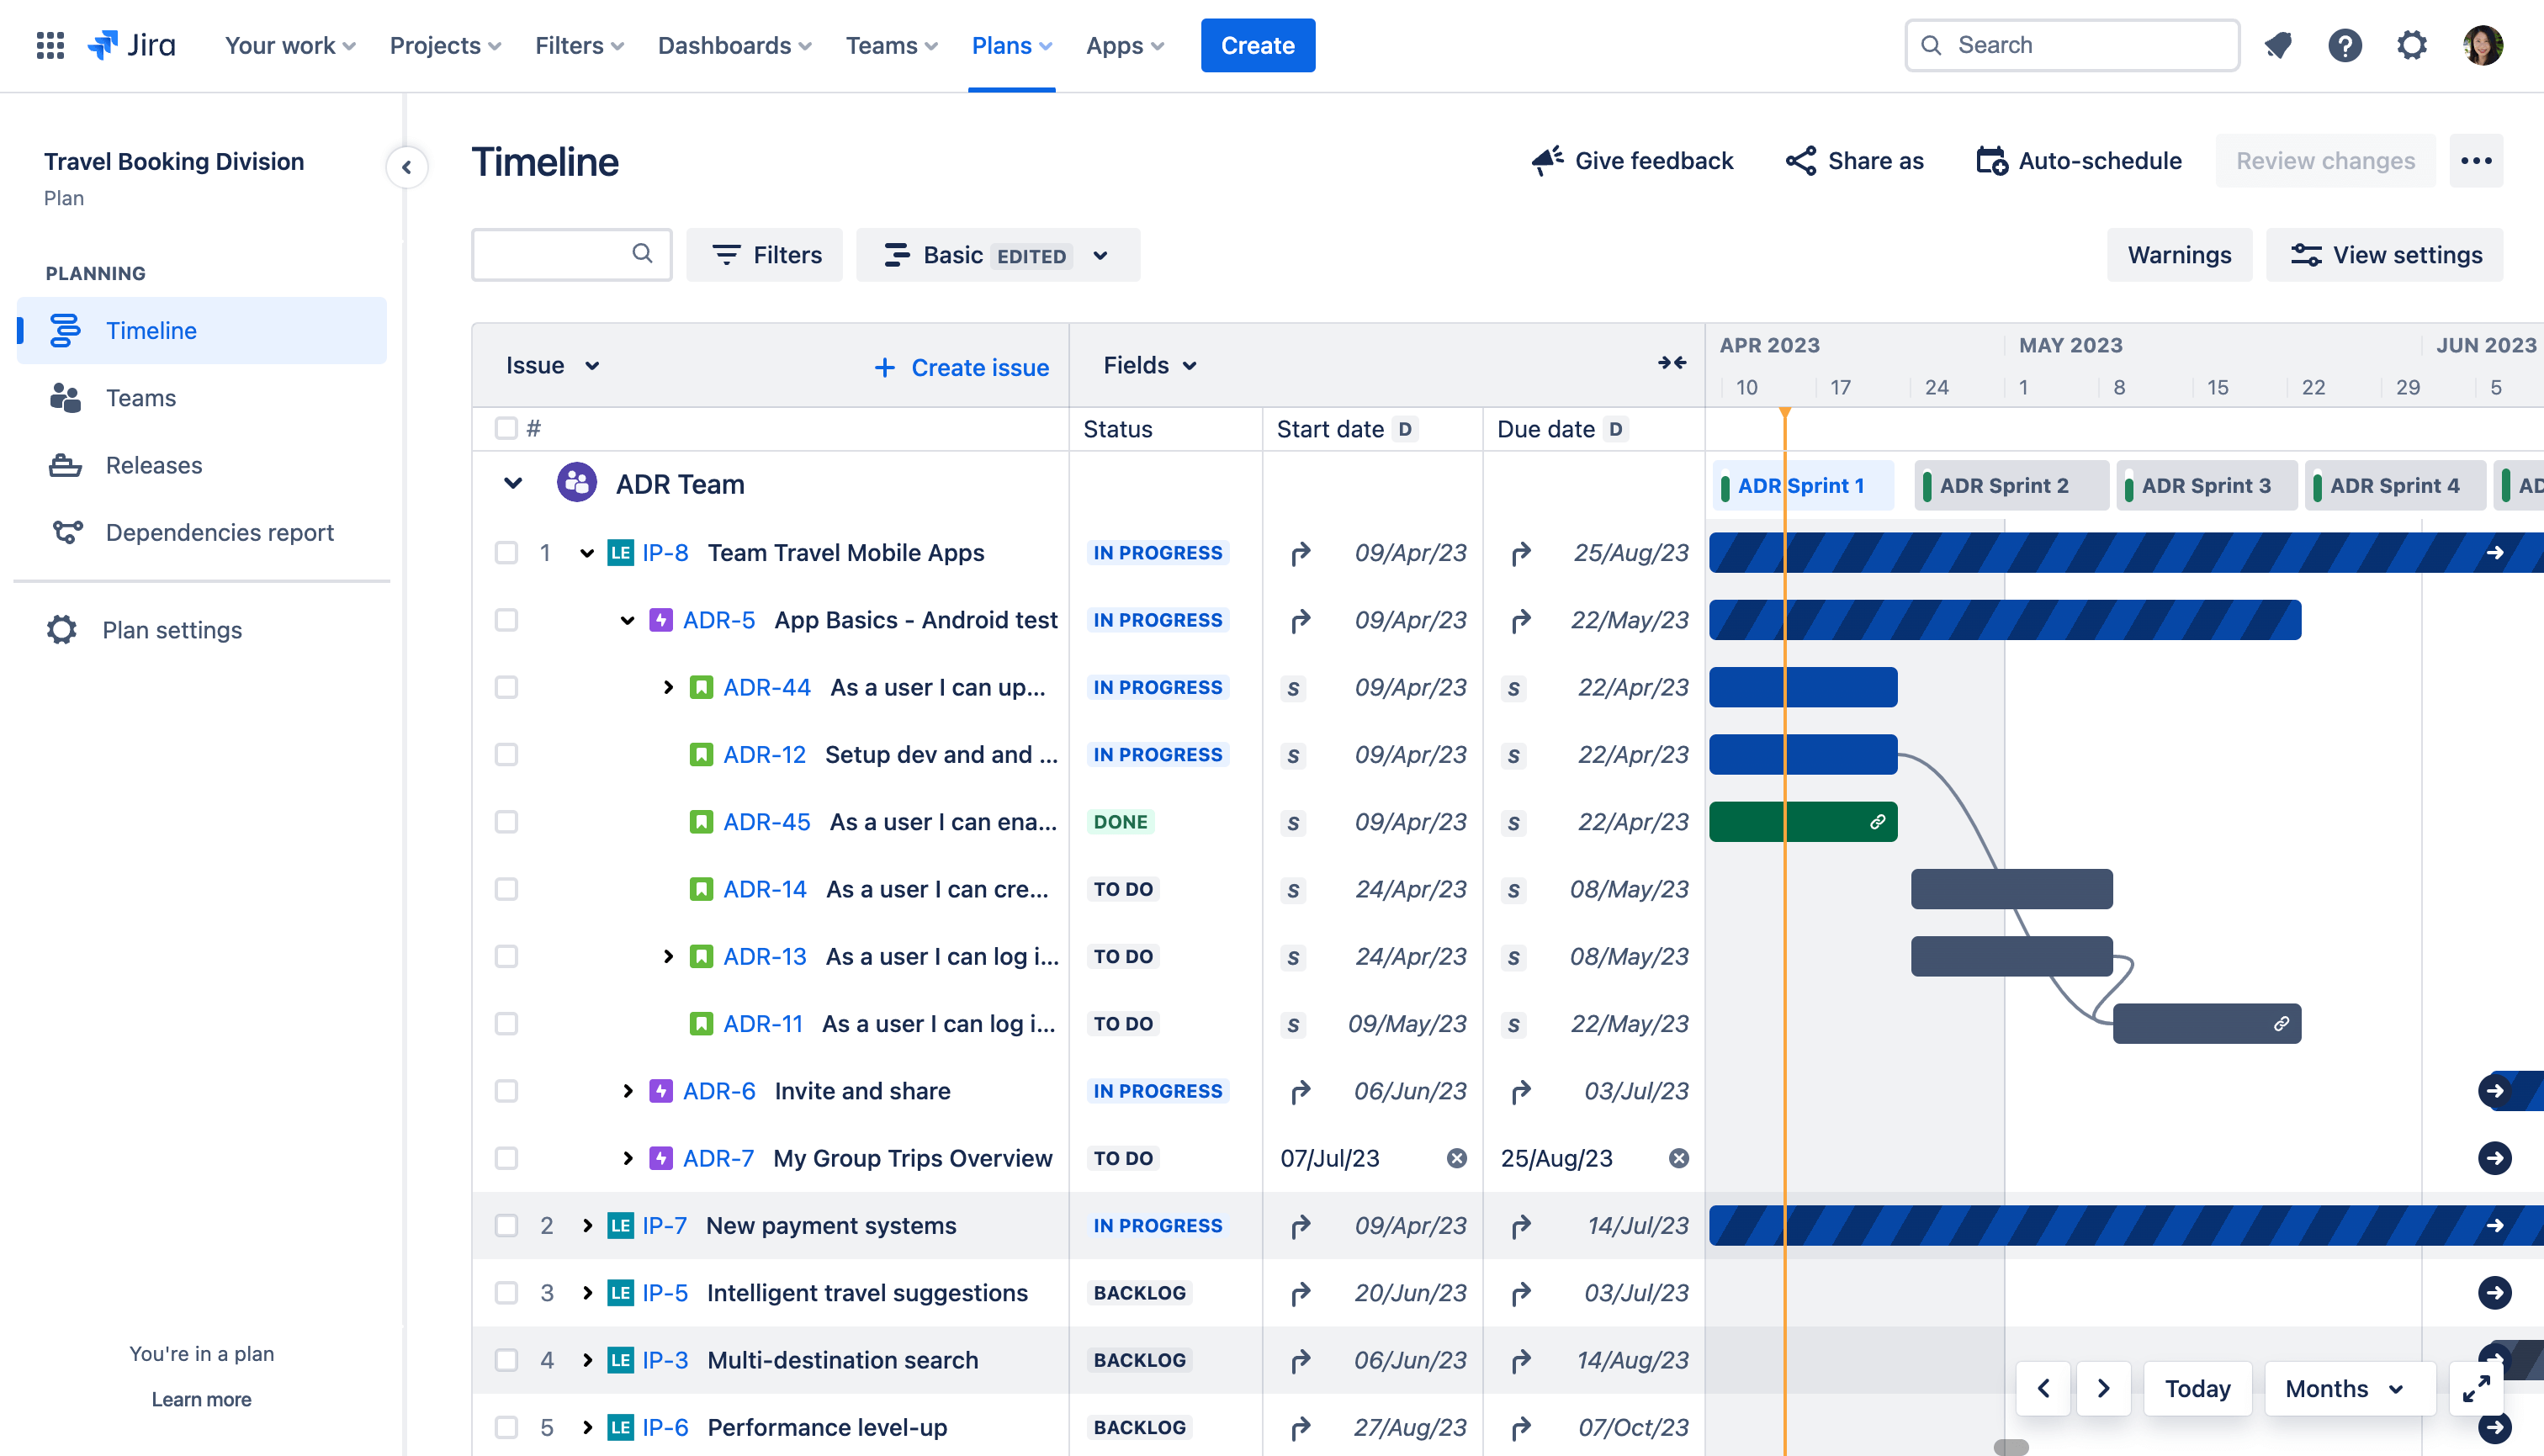
\includegraphics[alt={Esempio di gestione delle attività con \textit{Jira}}, width=0.7\columnwidth]{img/jira.png}
    \caption[Esempio di gestione delle attività con \textit{Jira}]{Esempio di gestione delle attività con \textit{Jira}\\ \textbf{Fonte:} \href{https://www.atlassian.com/it/software/jira/premium}{atlassian.com}}
    \label{fig:jira}
\end{figure}
\subsubsection*{Bitbucket}\noindent
Un'altro software nella suite di \textit{Atlassian} è \textit{Bitbucket}, che viene utilizzato per il controllo di versione e per la gestione del codice sorgente.
Con questo software è possibile creare \textit{repository}, questo spazio permette ai \textit{team} di collaborare in un modo efficiente, avendo anche la disponibilità di utilizzare funzionalità come le \gls{pullrequest}.
\begin{figure}[H]
    \centering
    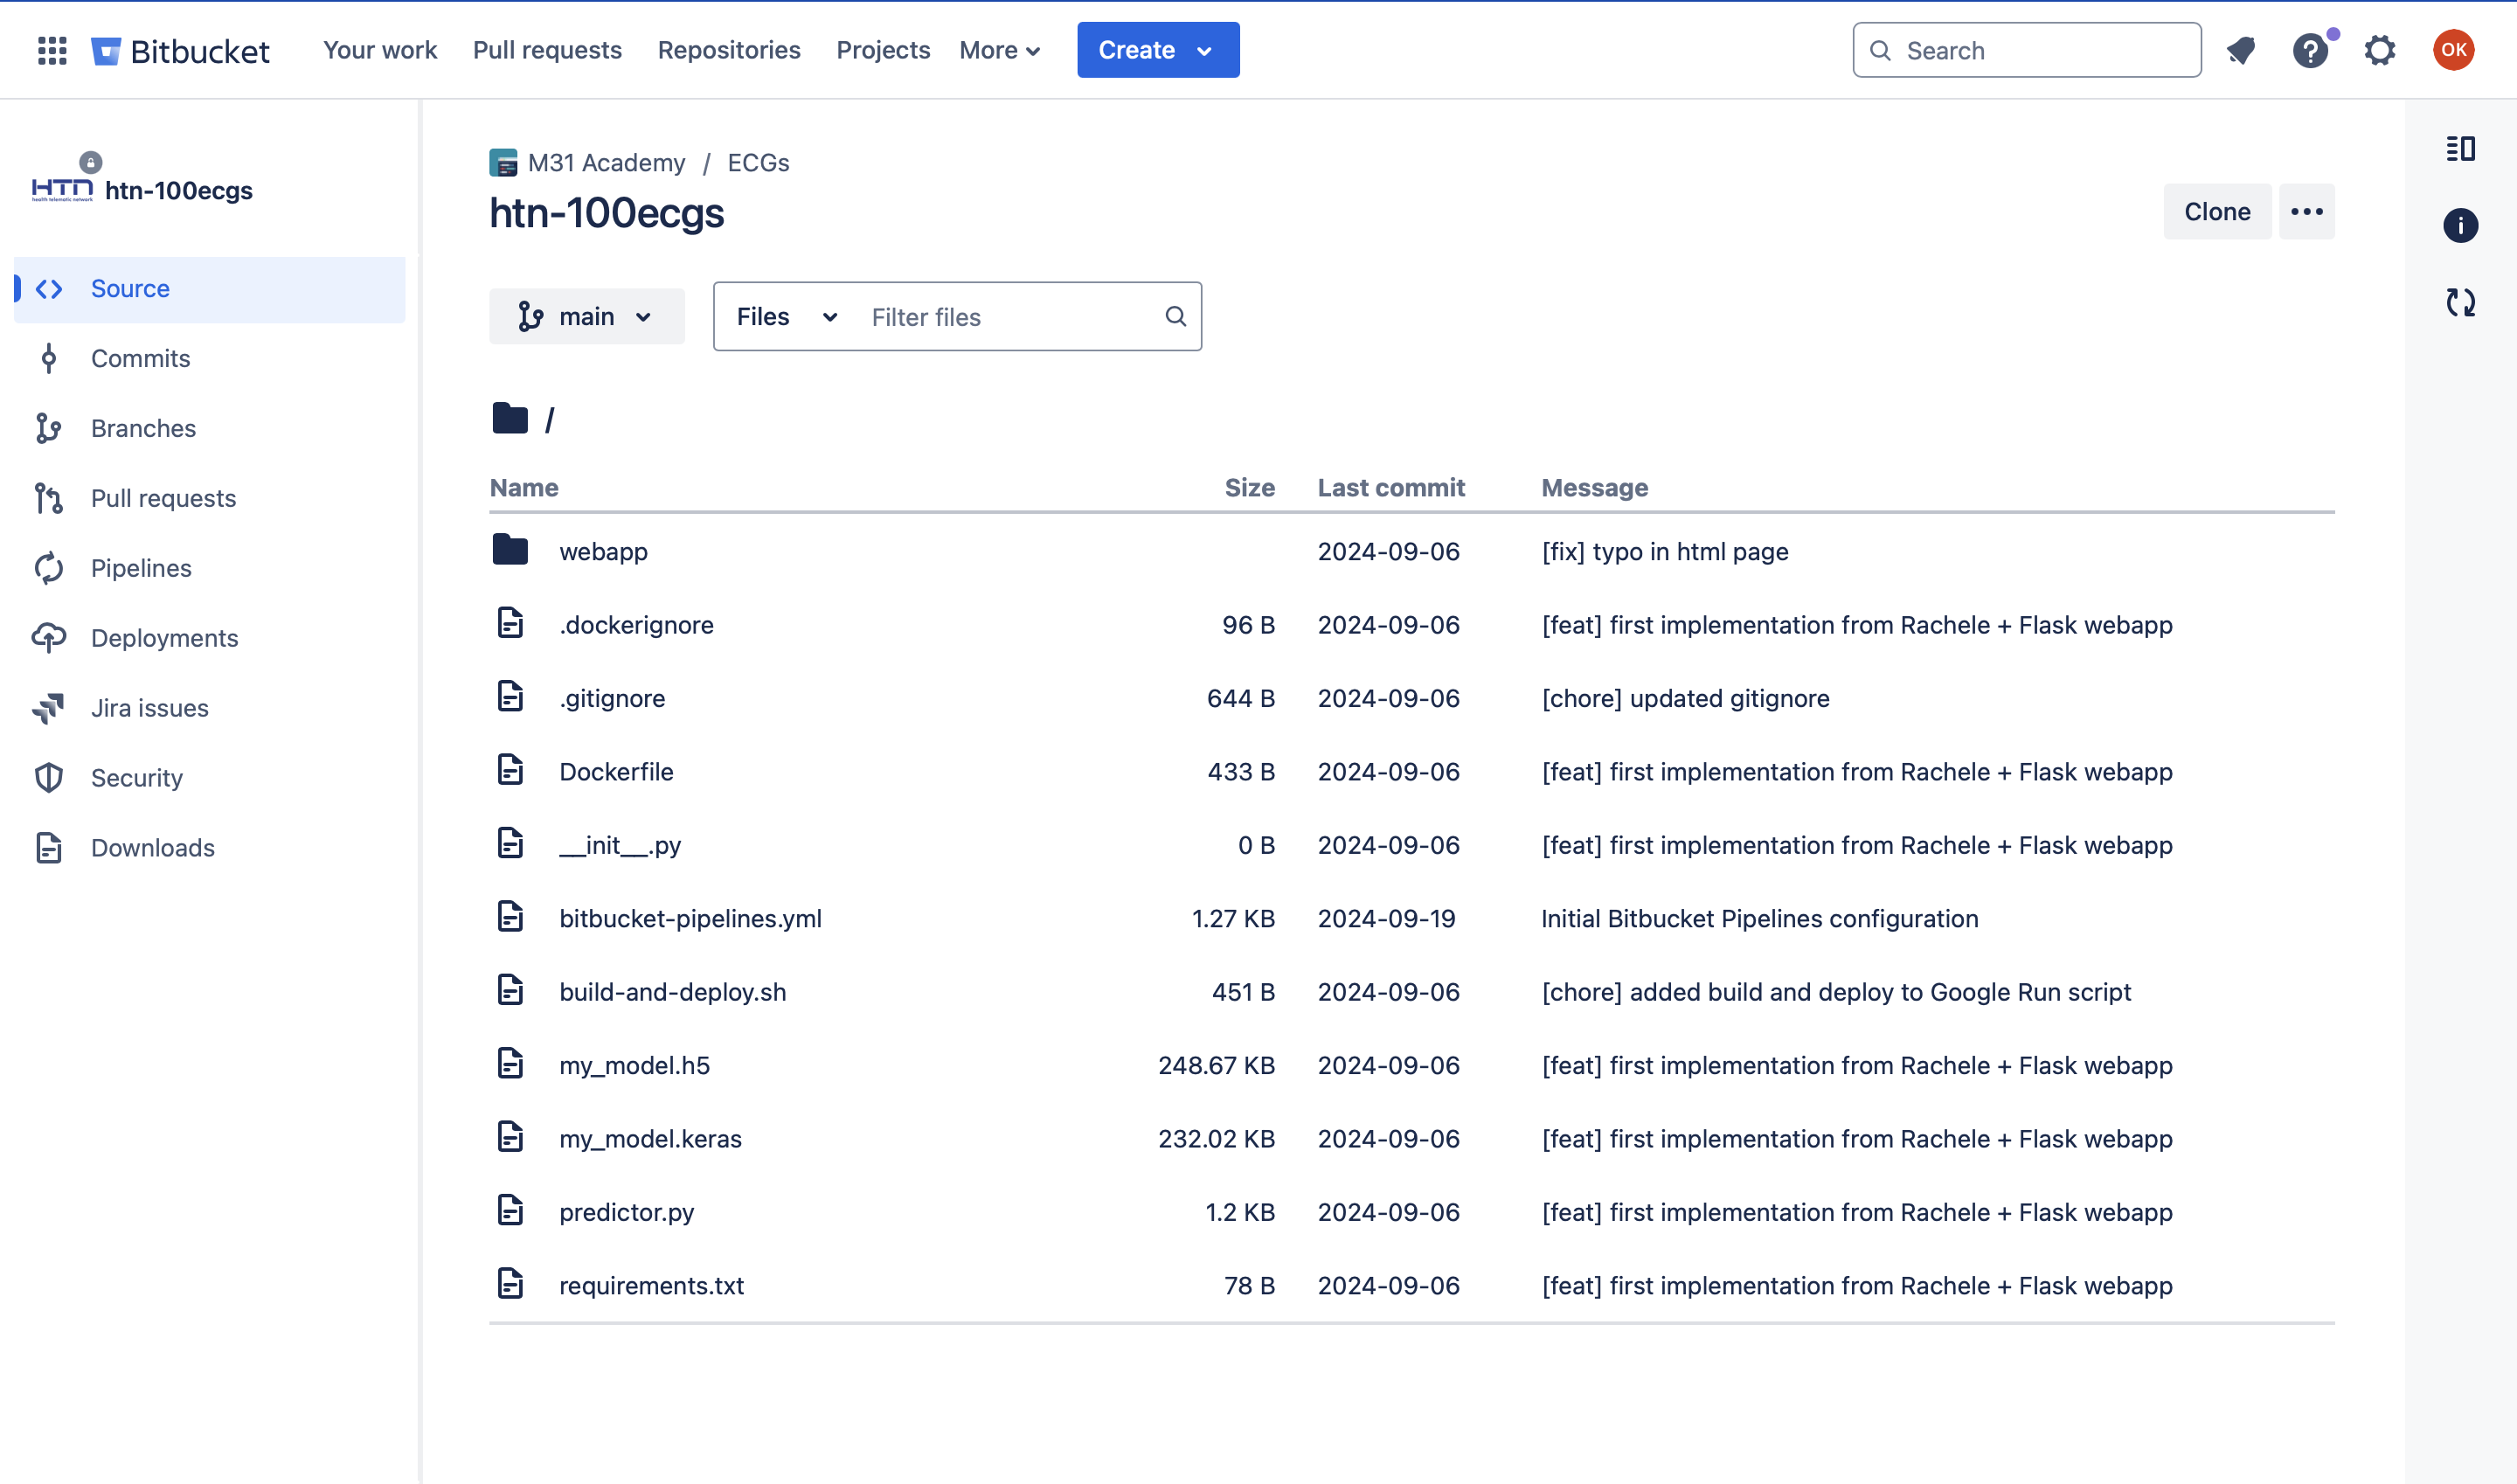
\includegraphics[alt={\textit{Screenshot} di una \textit{repository} in \textit{Bitbucket}}, width=0.9\columnwidth]{img/bitbucket.png}
    \caption{\textit{Screenshot} di una \textit{repository} in \textit{Bitbucket}}
    \label{fig:bitbucket}
\end{figure}
\subsubsection*{Confluence}\noindent
\textit{Confluence} è un'altro software sviluppato da \textit{Atlassian} e viene utilizzato per la gestione della documentazione.
Facendo parte della \textit{suite} di \textit{Atlassian} è ben integrato con le tecnologie precedentemente esposte.
All'interno di questo spazio vengono create documentazioni di prodotti e vari documenti contenenti risorse utili anche internamente.
\begin{figure}[H]
    \centering
    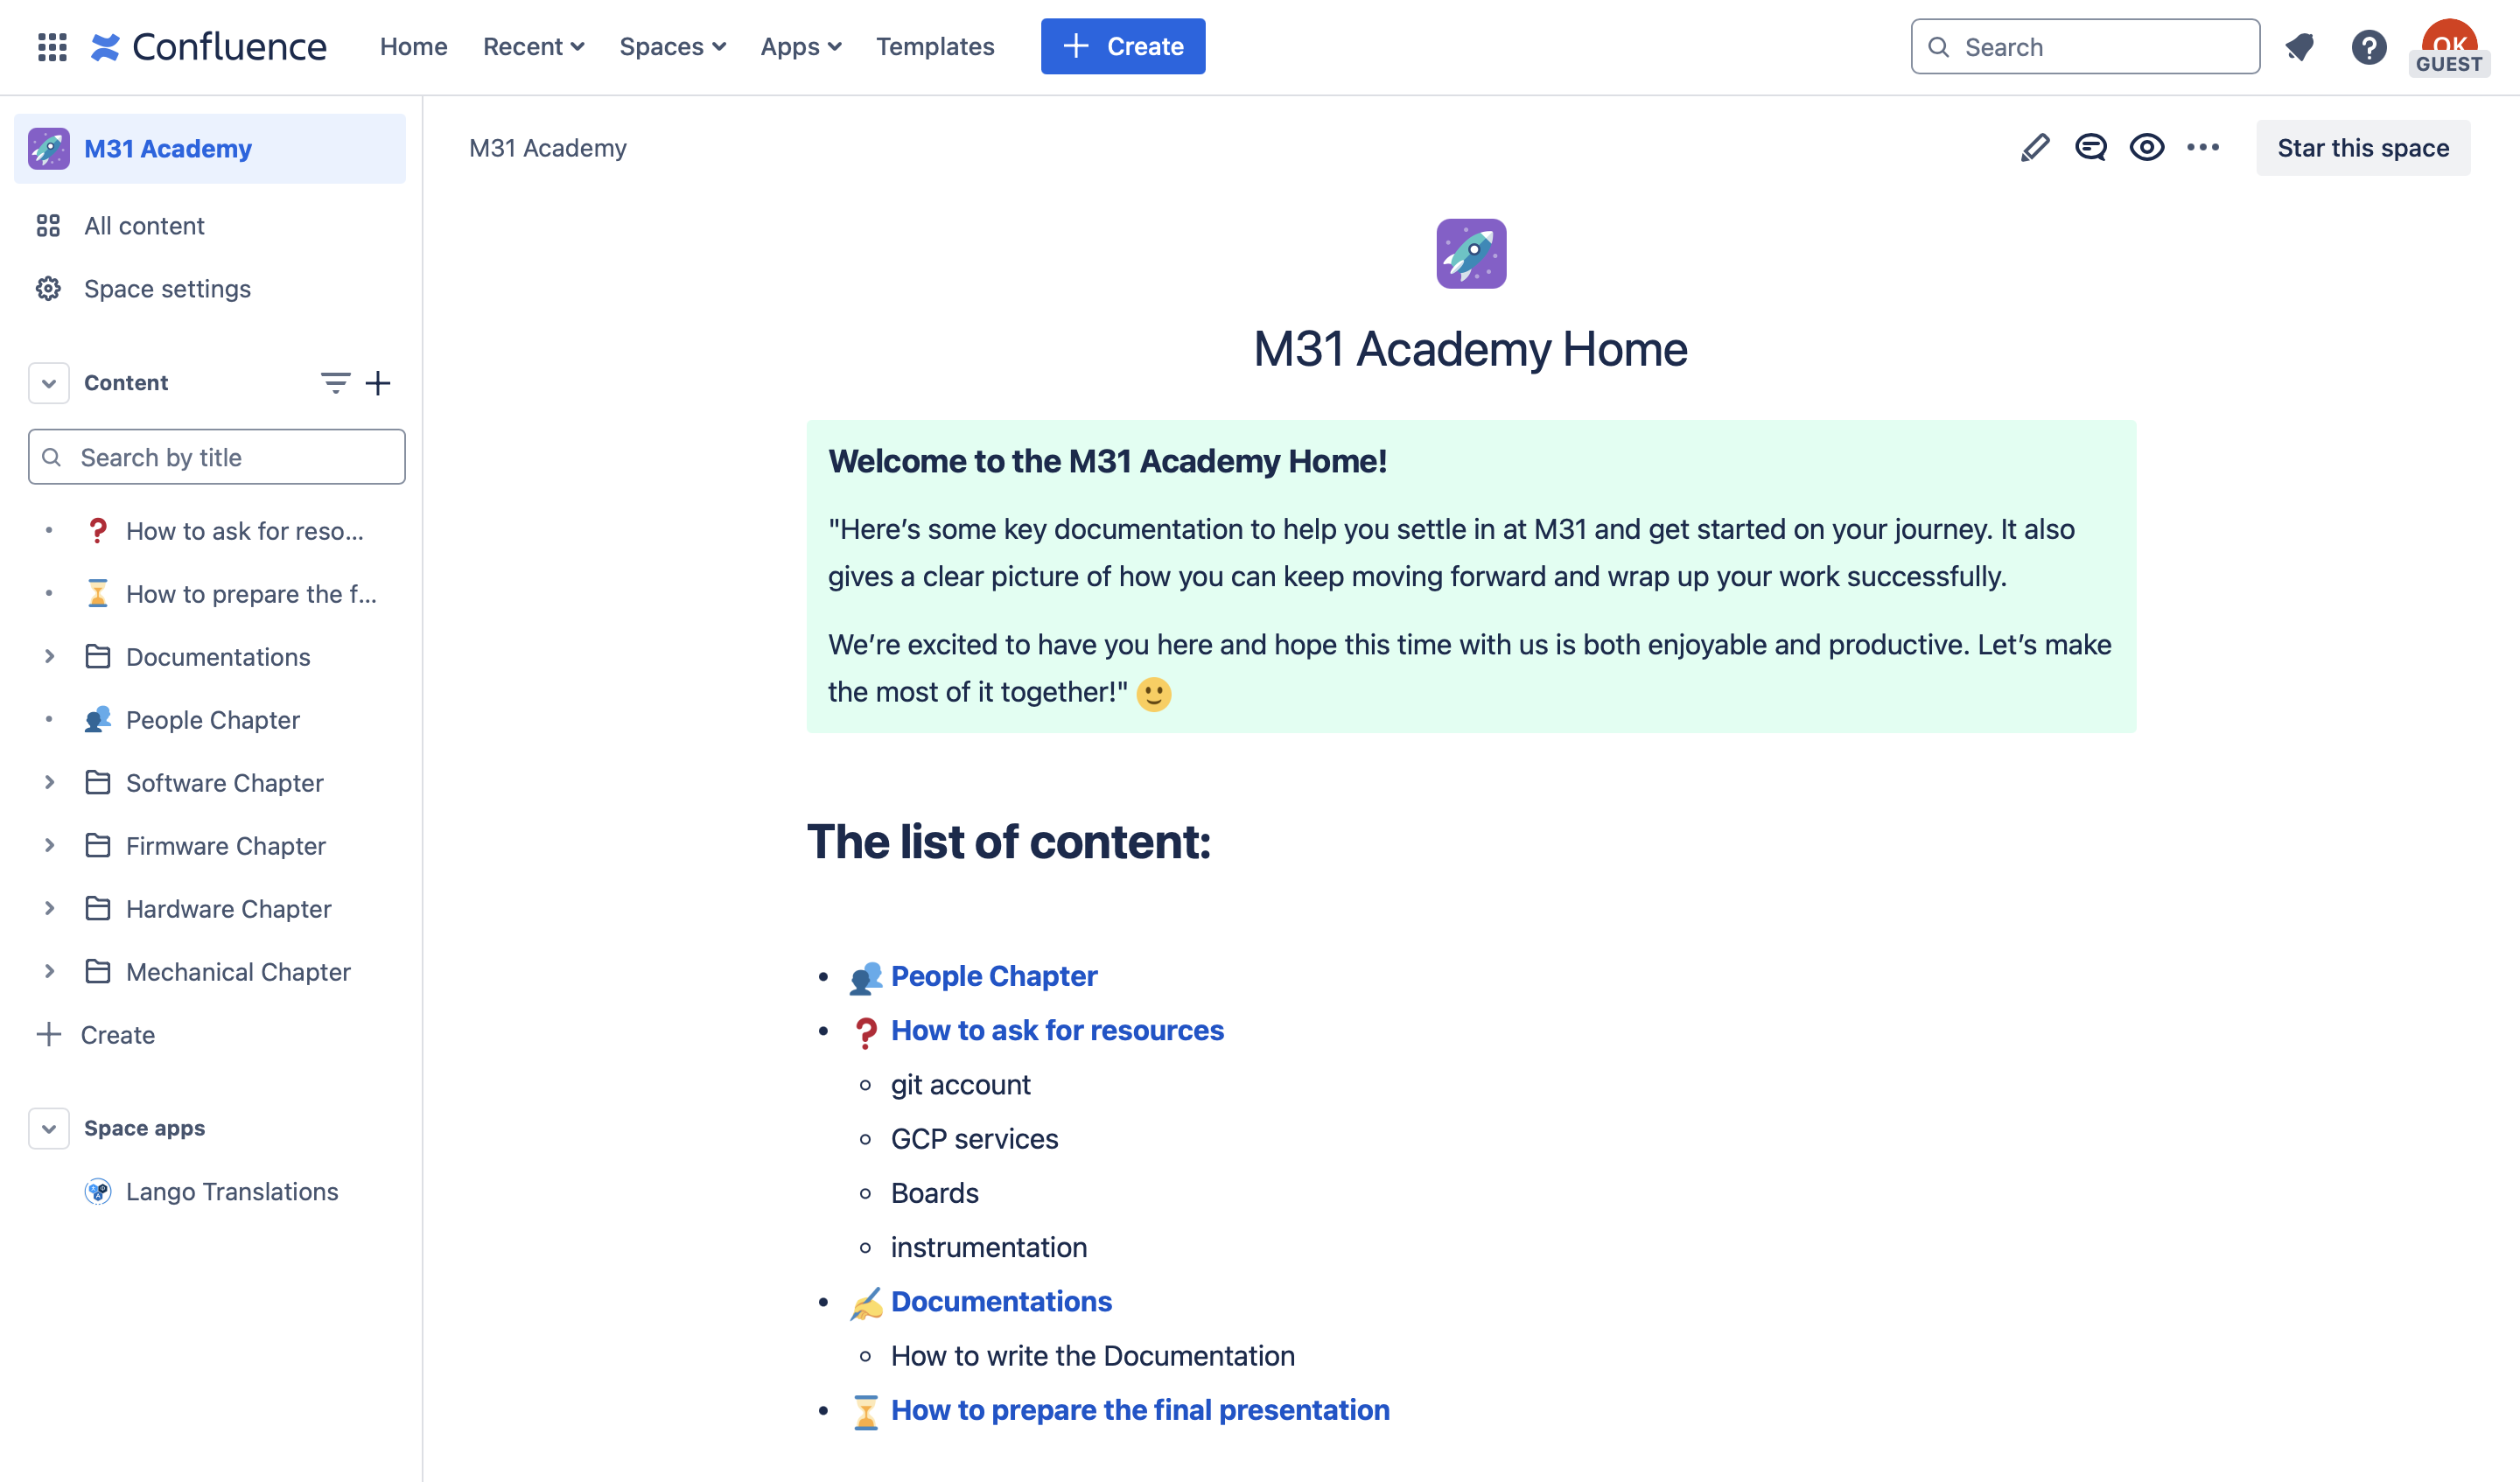
\includegraphics[alt={Pagina principale del \textit{Confluence} di M31 \textit{Academy}}, width=0.9\columnwidth]{img/confluence.png}
    \caption{Pagina principale del \textit{Confluence} di M31 \textit{Academy}}
    \label{fig:confluence}
\end{figure}
\subsubsection*{Microsoft Teams}\noindent
L'applicativo che viene utilizzato per comunicare è \textit{Microsoft Teams}. Questo software sviluppato da \textit{Microsoft} permette di comunicare, con singoli individui o con gruppi di persone, sia tramite messaggi testuali che tramite videochiamate.
Può essere usato anche per trasferimenti di piccoli file, ed è la prima opzione per comunicare con i membri dei team che lavorano da remoto.
\begin{figure}[H]
    \centering
    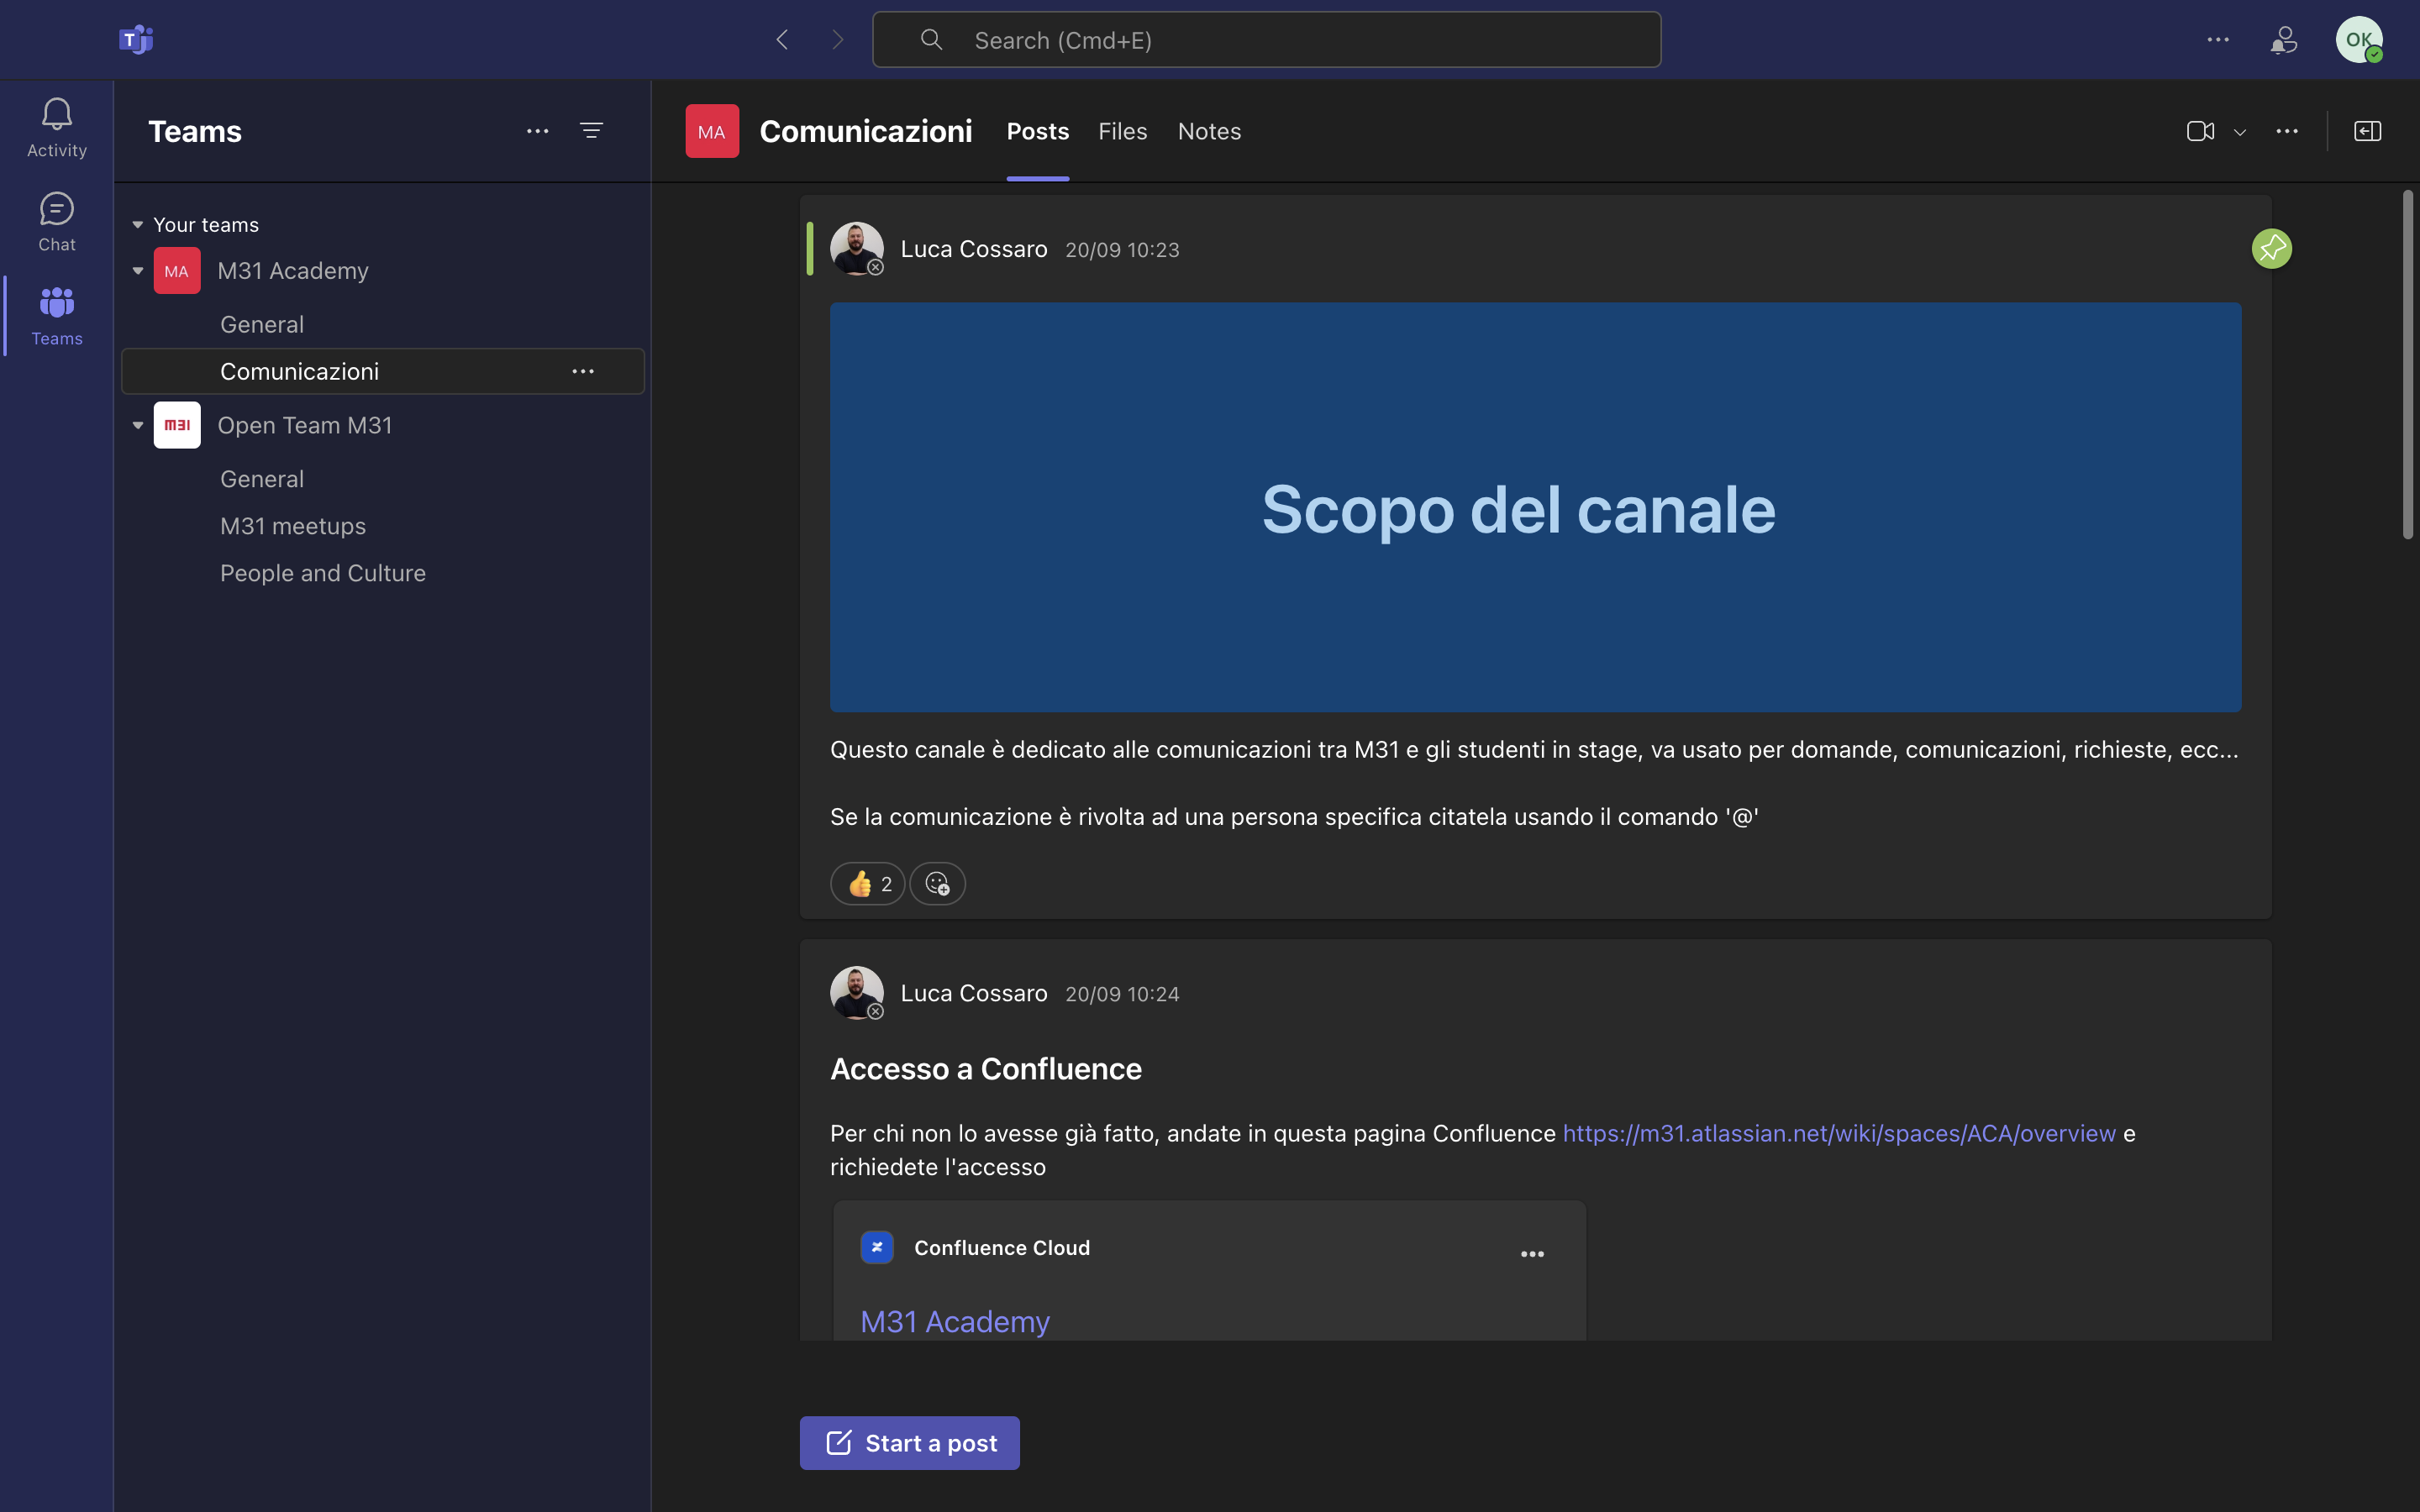
\includegraphics[alt={\textit{Screenshot} di un canale di comunicazione di M31 \textit{Academy}}, width=0.9\columnwidth]{img/microsoft-teams.png}
    \caption{\textit{Screenshot} di un canale di comunicazione di M31 \textit{Academy}}
    \label{fig:teams}
\end{figure}

% In questa sezione viene descritta come l'azienda si approccia con l'innovazione.
\section{Propensione all'innovazione}\label{sec:innovation}\noindent
M31 si interessa parecchio all'innovazione e questo lo si può vedere dalla filosofia con cui intraprende nuovi progetti di lavoro, come già menzionato nella sezione introduttiva \ref{sec:the-company}, i progetti che svolge sono tutti con lo scopo di portare progresso nei settori in cui si specializza.
Inoltre, durante lo svolgimento del mio tirocinio, ho potuto assistere ad un \textit{meeting} plenario che viene svolto periodicamente, nel quale ho potuto vedere in quali settori è l'azienda è intenzionata ad esplorare in futuro, sia dal lato della dirigenza che dal lato dei dipendenti.